\begin{titlepage}

	\begin{center}
		\begin{figure}[h]
			\centering
			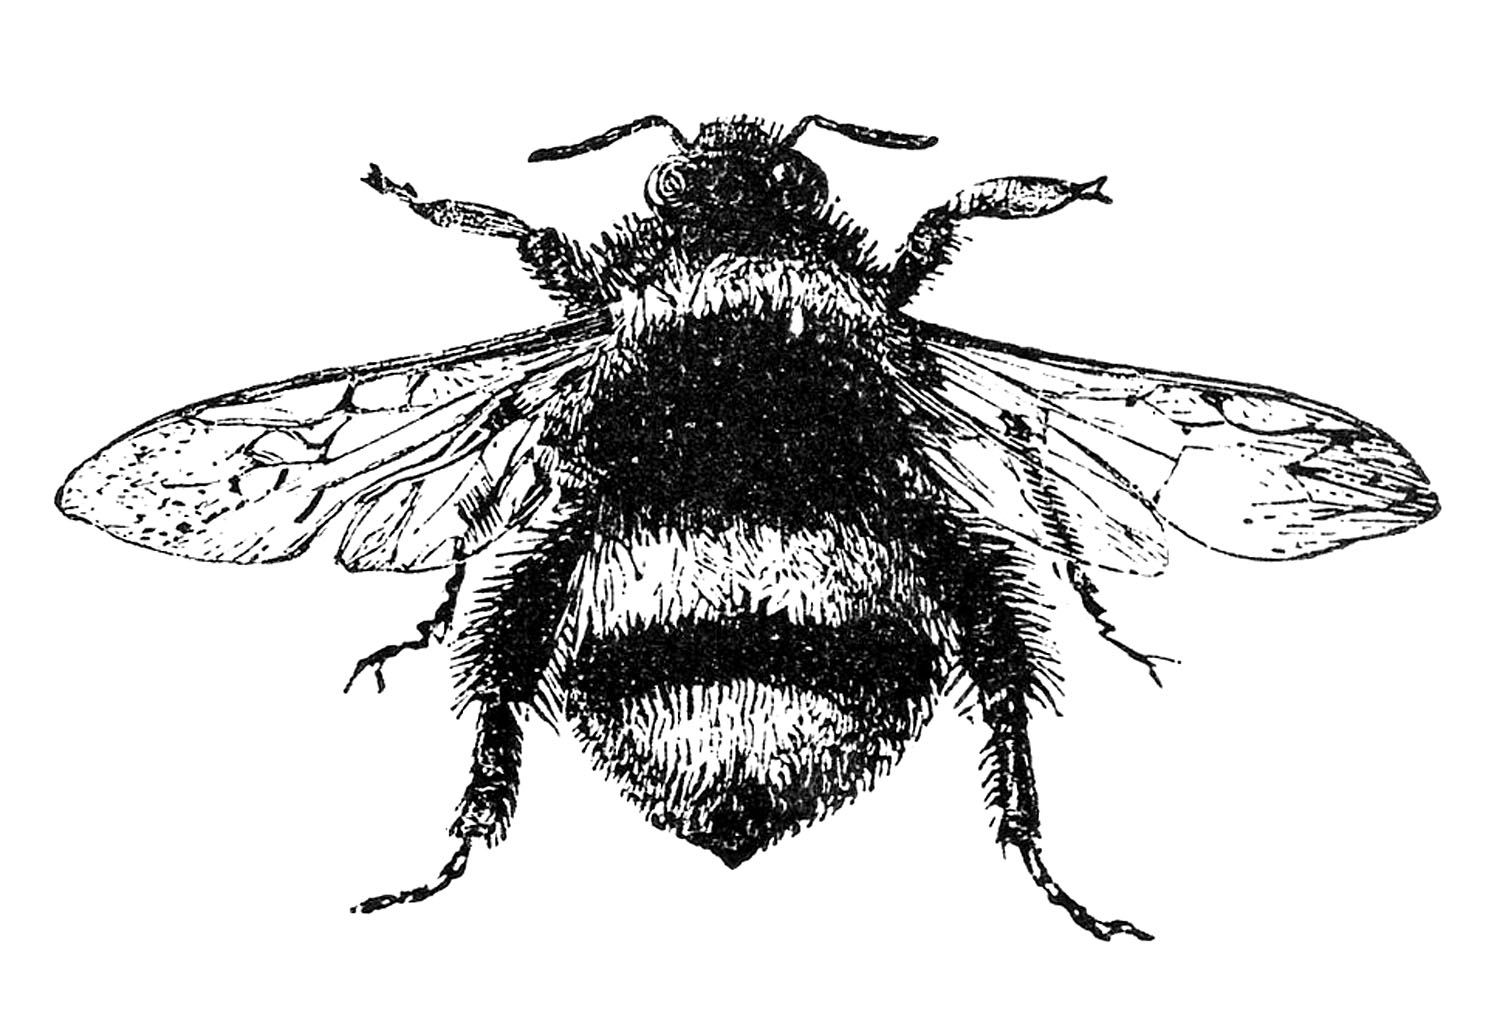
\includegraphics[scale=0.75]{img/bumblebee.jpg}
		\end{figure}
		\vspace{0.5cm}
		\Huge
		\textbf{\textsc{Metody Probabilistyczne Informatyki}}

		\vspace{0.5cm}
		\Large
		\textsc{Wybrane Dowody}

		\normalsize


		\line(1,0){330}

		\vspace{1cm}
		\textit{,,Tak teraz na to patrzę i myślę, czy ta nierówność nie powinna być w drugą stronę...''}
		\vspace{1cm}

		\textit{\textsc{Popełnione przez}}\\
		\vspace{5mm}

		\textbf{\textsc{
				Załatany Ponton \\
				V\\
				Nahtamatu\\
			}}

		\vfill

		Kraków \\
		Anno Domini 2025

	\end{center}

\end{titlepage}
